%++++++++++++++++++++++++++++++++++++++++
\documentclass[letterpaper,12pt]{article}
\usepackage[slovak]{babel}
\usepackage{tabularx} % extra features for tabular environment
\usepackage{amsmath}  % improve math presentation
\usepackage{graphicx} % takes care of graphic including machinery
\usepackage[margin=1in,letterpaper]{geometry} % decreases margins
\usepackage{cite} % takes care of citations

\usepackage[document]{ragged2e}

\usepackage{minted}
\usemintedstyle{borland}

\usepackage{algorithm2e,float}
\usepackage{varwidth}
\usepackage{amsfonts}
\usepackage{amsthm}
\usepackage{mathtools}

\usepackage[final]{hyperref} % adds hyper links inside the generated pdf file
\hypersetup{
	colorlinks=true,       % false: boxed links; true: colored links
	linkcolor=blue,        % color of internal links
	citecolor=blue,        % color of links to bibliography
	filecolor=magenta,     % color of file links
	urlcolor=blue         
}
\newtheoremstyle{dotless}{}{}{\itshape}{}{\bfseries}{}{ }{}
% \theoremstyle{dotless}
\newtheorem*{defn}{Definícia}
\newtheorem*{thm*}{Theorem}
%++++++++++++++++++++++++++++++++++++++++


\begin{document}
\title{\large \textbf{Komparatívna analýza vybraných \textit{reinforcement learning algoritmov} a ich výkonu v závisosti od zvolených parametrov \newline na jednoduchých \textit{OpenAI Gym} hrách}}
\author{Denisa Lampášová}
\date{\small \today}
\maketitle

\justify 
\begin{abstract}
TODO
\end{abstract}

\section{Úvod}

\indent\par Idea učenia algoritmu čisto na základe hodnotenia jeho správnania pozitívnym/negatívnym rewardom a skutočnosť, že sa tak naozaj dobre vedia naučiť napríklad hrať hry\footnote{\url{https://arxiv.org/pdf/1712.01815.pdf}} alebo nájsť vhodnú stratégiu pre obchodovanie s akciami\footnote{\url{https://arxiv.org/abs/1811.07522}} mi prišla veľmi fascinujúca. Tieto algoritmy nám taktiež poskytujú nové možnosti, ako sa naučiť niečo sami o sebe, napríklad akú výhodu majú predchádzajúce vedomosti pri hraní videohier\footnote{\url{https://www.youtube.com/watch?v=Ol0-c9OE3VQ}, prípadne samotný článok: \url{https://arxiv.org/pdf/1802.10217.pdf}.} alebo možnosť zistiť aké reward funkcie nás mohli viesť k naučeniu sa rôznych úkonov\footnote{\url{https://ai.stanford.edu/~ang/papers/icml00-irl.pdf}}. Bohužiaľ som nemala čas ani nápad na podobne dobrý výskum, ale chcela som sa aspoň poriadne naučiť základy reinforcement learningu a to spísaním teoretického úvodu a experimentovaním s rôznymi konceptami a algoritmami v tejto oblasti.

Konkrétne som sa rozhodla naimplementovať\footnote{Nie nutne from scratch. Teda aspoň pochopiť a použiť už existujúce implementácie algoritmov.} \textit{Value iteration, Policy iteration, Q-learning, SARSA}-u \textit{a Deep Q-learning} na natrénovanie agentov majúcich dobrý performance pri hraní jednoduchých \textit{OpenAI Gym} hier -- \textit{FrozenLake} a \textit{CartPole} a pohrať sa s tým, ako tieto algoritmy závisia od rôznych parametrov. Použité algoritmy sú dostupné tu: TODO.


\subsubsection*{FrozenLake}

\indent\par Je krásny zimný deň a s kamarátmi si hádžete frisbee v parku. Pri jednom nešťastnom hode sa ti však podarilo hodiť disk do stredu jazera. Našťastie je jazero z väčšej časti zamrznuté, ale je tam niekoľko dier, do ktorých nechceš spadnúť. Tvojou úlohou je dostať sa úspešne k disku. Ľad je ale klzký, takže nie vždy sa pohneš v zamýšľanom smere.

Hracia plocha je popísaná nasledujúcou mriežkou:
\begin{align*}
SFFF    \quad\quad\quad   &(S: \text{starting point, safe})\\
FHFH    \quad\quad\quad   &(F: \text{frozen surface, safe})\\
FFFH    \quad\quad\quad   &(H: \text{hole, fall to your doom})\\
HFFG    \quad\quad\quad   &(G: \text{goal, where the frisbee is located})
\end{align*}
Epizóda končí keď dorazíš k frisbee alebo spadneš do diery. Keď dorazíš k frisbee, získavaš reward +1, vo všetkých ostatných prípadoch je tvoj reward 0.

\subsubsection*{CartPole (Inverted pendulum)}

\indent\par Máme vozidlo, na ktorom je pripevnené inverzné kyvadlo. Aplikovaním sily +1 alebo -1 (iná možná akcia nie je) ovládame pohyb tohoto vozidla po 1 rozmernej čiare (bez trenia). Začiatočný stav (poloha vozidla, rýchlosť vozidla, uhol vychálenia tyče, uhlová rýchlosť tyče) je náhodne inicializovaný medzi +/-0.05 a našim cieľom je zabrániť prevráteniu kyvadla. Za každý časový krok, kedy sa kyvadlo ešte neprevrátilo dostávame odmenu +1. Epizóda končí, keď je tyč vychýlená o viac než $15^\circ$ (= keď sa kyvadlo prevrátilo) alebo keď sa vozidlo vzdiali viac než 2.4 jednotiek od stredu.

\begin{figure}[H]
\centering
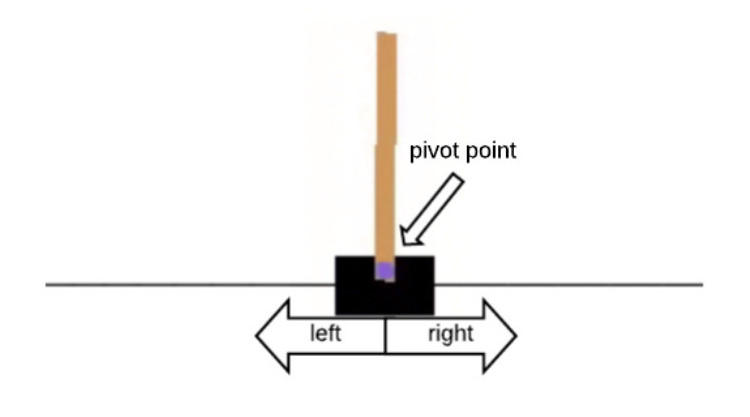
\includegraphics[width=9cm]{images/cartpole.jpg}
\caption{Ilustrácia CartPole systému.}
\end{figure}


\section{Reinforecement Learning - theoretical background}
\subsubsection*{Markov Decision Process (MDP)}
\begin{figure}[H]
\centering
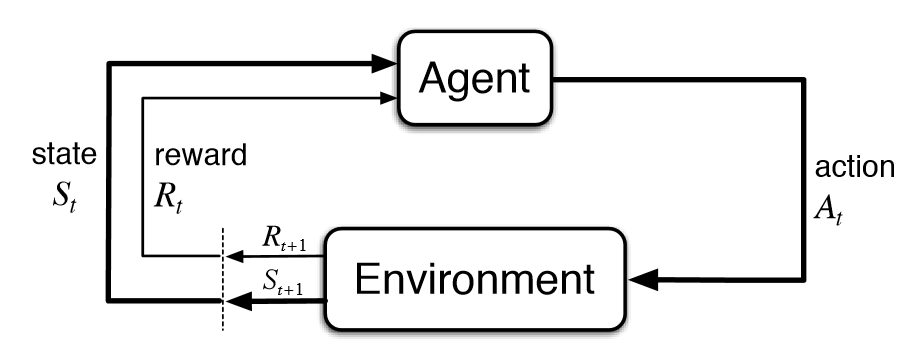
\includegraphics[width=12cm]{images/rl-diagram.png}
\caption{Schéma MDP.}
\label{rl-diagram}
\end{figure}

\indent\par Agent (decision maker) interaguje s prostredím nasledovne (viď Obr. \ref{rl-diagram}). V každom časovom kroku $t$ agent obdrží nejakú reprezentáciu stavu prostredia $s_t$. Na základe tohto stavu sa agent rozhodne, ktorú akcu $a_t$ v tomto kroku vykoná. Po vykonaní tejto akcie sa stav prostredia zmení na $s_{t+1}$ a agent ako následok za jeho akciu obdrží nejaký reward $r_{t+1}$. Dostávame sa do ďaľšieho časového kroku a celý proces sa opakuje.

Celkovo teda vytvárame istú postupnosť
$$s_0 \xrightarrow[]{a_0} s_1 \xrightarrow[]{a_1} s_2 \xrightarrow[]{a_2} s_3 \xrightarrow[]{a_3} \cdots,$$
v ktorej sa kumuluje celkový reward
\begin{align*}
R = r_{1} + r_{2} + r_3 + \cdots.
\end{align*}
Cieľom agenta je tento reward maximalizovať. Nakoľko je ale často predpovedanie blízkeho rewardu presnejšie, ňež krokovo vzdialenejšieho rewardu a teda, napríklad, ak má agent možnosť vybrať si, či dostane odmenu (dolár) v najbližšom kroku (dnes) alebo až v tom ďalšom (zajtra), chceme aby sa vždy rozhodol pre najbližší krok. Dolár dnes je predsa cennejší než dolár zajtra. Preto zavádzame \textit{discount faktor} $\gamma$ a agent sa snaží maximalizovať \textit{discounted cummulative reward}
\begin{align*}
G_t &= r_{t+1} + \gamma \cdot r_{t+2} + \gamma^2 \cdot r_{t+3} + \cdots = \sum\limits_{k=0}^\infty \gamma^k \cdot r_{t+k+1}\\
	&= r_{t+1} + \gamma G_{t+1}.
\end{align*}
Ďalšou výhodou je, že ak má agent na výber dlhšiu cestu s väčším rewardom a kratšiu cestu s menším rewardom, vieme výberom $\gamma$ ovplyvniť, ktorú trasu má zvoliť. 

\begin{defn}
Markov Desicion Process je 5-tica $\left(S, A, \{ P_{sa} \}, \gamma, R\right)$, kde:

\begin{itemize}
\item $S$ je množina \textbf{stavov} (v prípade FrozenLake-u je to id políčka, na ktorom agent stojí.)
\item $A$ je množina \textbf{akcií} (Napríklad smery ktorými sa môže agent pohnúť - hore, dole, doľava a doprava.)
\item $p\big(s'\,|\,s, a\big)$ are the \textbf{state transition probabilities} - pravdepodobnosť, že sa dostaneme do stavu $s'$, ak v stave $s$ vykonáme akciu $a$. Môžeme sa na to pozerať aj ako na pravdepodobnostnú distribúciu nad možnými stavmi $s'$, do ktorých nás vie dostať akcia $a$ zo stavu $s$. (Napríklad vo FrozenLake-u je plocha šmykľavá a preto je nejaká pravdepodobnosť, že my síce zvolíme akciu doprava, ale v skutočnosti sa pohneme napríklad na políčko nad nami.)
\item $\gamma \in [0,1]$ je discount faktor,
\item $R: S \to \mathbb{R}$ je \textbf{reward funkcia} (všeobecnejšie sa definuje ako $R: S \times A \to \mathbb{R}$ - môžeme agenta odmeňovať aj za zvolenie niektorej akcie, nie nutne len za skončenie v niektorom stave).
\end{itemize}
\end{defn}

Ako ale určiť, ako dobrý je pre agenta nejaký stav alebo akcia? A ako presne sa agent v stave $s$ rozhoduje, ktorú akciu zvolí?
Zaveďme si na to teda terminológiu a zodpovedajme tieto otázky.

\subsubsection*{Policy}

\indent\par Policy je ľubovoľná funkcia $\pi: S \to A$. Úlohou agenta je rozhodnúť sa na základe stavu $s$, ktorú akciu $a$ zvolí. Policy slúži presne na popis týchto rozhodnutí - hovoríme potom, že agent nasleduje/riadi sa policy $\pi$.

\subsubsection*{Value function}
\begin{itemize}
	\item \textbf{State-value function} {\boldmath $v_\pi(s)$} nám hovorí, ako dobrý je nejaký stav $s$ pre agenta nasledujúceho policy $\pi$
$$v_\pi(s) = \mathrm{E}\big[G_t|s_t = s\big].$$
		\item \textbf{Action-value function} (alebo tiež \textbf{Q-function}) {\boldmath $q_\pi(s,a)$} evaluuje, ako dobré je pre agenta v stave $s$ nasledujúceho policy $\pi$ zvoliť akciu $a$
$$q_\pi(s,a) = \mathrm{E}\big[G_t|s_t = s, a_t = a\big].$$
\end{itemize}

\begin{thm*}[Bellman equations]
Majme MDP $M = \left(S, A, \{ P_{sa} \}, \gamma, R\right)$ a policy $\pi: S \to A$. Potom pre všetky $s \in S$, $a \in A$, $v_\pi$ a $q_\pi$ spĺňajú 
\begin{align*}
v_\pi (s) &= \sum\limits_{s'} p\big(s'\,|\,s, \pi(s)\big) \cdot \big(R(s') + \gamma \cdot v_\pi (s')\big)\\
 &= \mathrm{E}\big[r|s, \pi(s)\big] + \gamma \sum_{s' \in S} p(s'|s,\pi(s)) \cdot v^\pi(s'),\\
q_\pi (s,a) &= \sum\limits_{s'} p\big(s'\,|\,s, a\big) \cdot \big(R(s') + \gamma \cdot v_\pi (s')\big)\\
 &= \mathrm{E}\big[r|s,a\big] + \gamma \sum_{s' \in S} p(s'|s,a) \cdot v^\pi(s').
\end{align*}
\end{thm*}
\noindent Tieto vzťahy sa ukážu byť veľmi užitočné (napríklad vo value a policy iteration algoritmoch), nakoľko nám navrhujú spôsob ako iteratívne vypočítať hodnoty $v_\pi$ a $q_\pi$.

\subsubsection*{Optimal policy}
\indent\par Cieľom reinforcement learningu je nájsť \textbf{optimálnu policy} {\boldmath $\pi^\star$}. Hovoríme, že policy $\pi$ je lepšia/optimálnejšia než policy $\pi'$  ($\pi \geq \pi'$) práve vtedy, keď $v_\pi(s) \geq v_{\pi'}(s)$ pre všetky $s \in S$. Nuž a optimálna policy je lepšia než akákoľvek iná možná policy.

K optimálnej policy prislúcha aj \textbf{optimálna state-value funkcia} {\boldmath $v_\star$}
$$v_\star (s) = \max\limits_{\pi} v_\pi(s) \quad (\forall s \in S),$$
čo je vlastne najlepšia možná očakávaná hodnota discounted cummulative rewardu od toho momentu, ktorá vie byť dosiahnutá.
Môžeme taktiež definovať \textbf{optimálna action-value funkcia} {\boldmath $q_\star$} ako
$$q_\star (s,a) = \max\limits_{\pi} q_\pi(s,a) \quad (\forall s \in S, \forall a \in A),$$
ktorá nám zas hovorí, aká je najlepšia možná očakávaná hodnota discounted cummulative rewardu potom, čo v stave $s$ vykonáme akciu $a$.

\begin{thm*}[Bellman optimality]
Majme MDP $M = \left(S, A, \{ P_{sa} \}, \gamma, R\right)$ a policy $\pi: S \to A$. Potom $\pi$ je optimálna policy práve vtedy, keď pre všetky $s \in S$
\begin{align*}
\pi (s) \in \arg\max\limits_{a \in A} q_\pi(s,a).
\end{align*}
\end{thm*}

\noindent Celkovo je teda zrejmé, že
\begin{align*}
v_\star (s) &= \max\limits_{a} q_\star (s,a),\\
v_\star (s) &= \max\limits_{a} \Big[\sum\limits_{s'} p\big(s'\,|\,s, a\big) \cdot \big(R(s') + \gamma \cdot v_\star (s')\big)\Big],\\ 
q_\star(s,a) &= E\Big[r_{t+1} + \gamma \max\limits_{a'} q_\star(s',a')\Big] = \sum\limits_{s'} p\big(s'\,|\,s, a\big) \cdot \big(R(s') + \gamma \cdot v_\star (s')\big),
\end{align*}
kde posledné dve rovnice sa nazývajú \textbf{Bellman optimality equations}. Teraz máme už slušný teoretický základ a môžeme sa pozrieť na základné algoritmy.


\section{Reinforcement learning - algoritmy}
\subsection{Value iteration}

\indent\par Value iteration počíta optimálnu state-value function tak, že najskôr zinicializuje $v(s)$ na nuly a potom iteratívne, pomocou Bellman optimality equation, vylepšuje hodnoty $v(s)$, kým nezkonvergujú. Keď už máme $v_\star$, vieme jednoducho (použitím Bellman otimality theorem) získať optimálnu policy $\pi^\star$. Pseudokód:

\vspace{0.3cm}
\begin{algorithm}[H]
\noindent\fbox{%
\begin{varwidth}{\dimexpr\linewidth-2\fboxsep-2\fboxrule\relax}
\begin{algorithm}[H]
 Initialize $v(s)$ to arbitrary values (usually 0s)\;
 \Repeat{$v(s)$ converges}{
 	\For {all $s \in S$}{
 		\For {all $a \in A$}
  			{$q(s,a) \gets \mathrm{E}\big[r|s,a\big] + \gamma \cdot \sum_{s' \in S} p(s'|s,a) \cdot v(s')$\;}{}{}
 	 	$v(s) \gets \max_a q(s,a)$\;}{}{}}
  
\end{algorithm}
\end{varwidth}% 
}
\vspace{0.4cm}
\caption{Pseudocode for value iteration algorithm.}
\end{algorithm}
\vspace{0.3cm}

Máme ale 2 možnosti, ako update-ovať $v(s)$ vo vnútornom \textit{for}-cykle.
\begin{enumerate}
	\item V každej iterácii (repeat till $v(s)$ converges), najskôr pre všetky $s \in S$ vypočítame $v(s)$ a až potom sunchrónne prepíšeme všetky hodnoty. Takýto spôsob voláme \textbf{synchronous} update.
	\item Môžeme použiť aj \textbf{asynchronous} update, kedy pre každý stav $s \in S$, hneď ako zistíme novú hodnotu $v(s)$, ju priamo aj prepíšeme. Nečakáme kým, zistíme ostatné. 
\end{enumerate}

V oboch prípadoch sa dá ukázať, že $v$ naozaj skonverguje do $v_\star$. Nevýhodou tohoto algoritmu je ale predpoklad, že vlastnosti prostredia už poznáme. Tieto vlastnosti nám ale nie sú vždy popredu známe (potom ich samozrejme je možné nejako odpozorovať, ale získame tým nejaké nepresnosti). Taktiež, priamočiaro vieme tento algoritmus použiť len pre prípady s diskrétnou množinou stavov $S$ (ako je napríklad vo FrozenLake-u). Pre prípad so spojitou množinou stavov $S$ (ako je napríklad v CartPole-e), je potrebné túto množinu diskretizovať, čo môže zapríčiniť, že policy, ktorú získame, už nebude optimálna.

\subsection{Policy iteration}

Value iteration algoritmus vylepšuje hodnoty $v(s)$ až kým neskonverguje. Ale všetko, čo agent potrebuje vedieť je len optimálna policy. Niekedy sa stáva, že optimálna policy zkonverguje skôr než value funkcia. Policy iteration algorithm teda miesto opakovaného vylepšovania hodnôt value funkcie, v každom kroku redefinuje policy. Na základe tejto novej policy potom iteratívne vypočíta príslušnú state-value funkciu $v_\pi$. Podľa vypočítanej value funkcie potom opäť predefinuje policy a proces sa opakuje, kým policy neskonverguje. Pseudokód:

\vspace{0.3cm}
\begin{algorithm}[H]
\noindent\fbox{%
\begin{varwidth}{\dimexpr\linewidth-2\fboxsep-2\fboxrule\relax}
\begin{algorithm}[H]
 Initialize a policy $\pi'$ arbitrarily\;

 \Repeat{$\pi = \pi'$}{
 	1. $\pi \gets \pi'$\;
 	2. Iteratively evaluate the value-function under policy\\
 	(for all states, till $v^\pi$ converges):\\
 	\vspace{0.1cm}
 	$v^{\pi}(s) = \mathrm{E}\big[r|s, \pi(s)\big] + \gamma \sum_{s' \in S} p(s'|s,\pi(s)) \cdot v^\pi(s')$\;
 	\vspace{0.1cm}
 	3. Improve the policy at each state:\\
 	\vspace{0.1cm} 	
 	$\pi'(s) \gets \arg\max_{a}(\mathrm{E}\big[r|s,a\big] + \gamma \sum_{s' \in S} p(s'|s,a) \cdot v^\pi(s'))$\;
 	\vspace{0.1cm} 	
 	}
\end{algorithm}
\end{varwidth}% 
}
\vspace{0.4cm}
\caption{Pseudocode for policy iteration algorithm.}
\end{algorithm}
\vspace{0.3cm}

Policy iteration tiež zaručenie skonverguje k optimálnej policy a často jej zkonvergovanie trvá menej iterácií než value iteration algoritmu, každá z týchto iterácií je ale výpočtovo náročnejšia. Taktiež tu platia rovnaké problémy s diskretizáciou a nevedomosťou prechodových pravdepodobností a raward funkciou.


\subsection{Q-learning}

Prvou výhodou tohto algoritmu je, že nepredpokladá, že agent pozná efekty jeho akcií popredu. Agent pozná iba množinu možných stavov $S$ a akcií $A$. Na ich základe si na začiatku vytvorí a inicializuje \textbf{q-table} na nuly. Následne chceme postupne update-ovať hodnoty (action-value funkcie) v tabuľke. 

\begin{figure}[H]
\centering
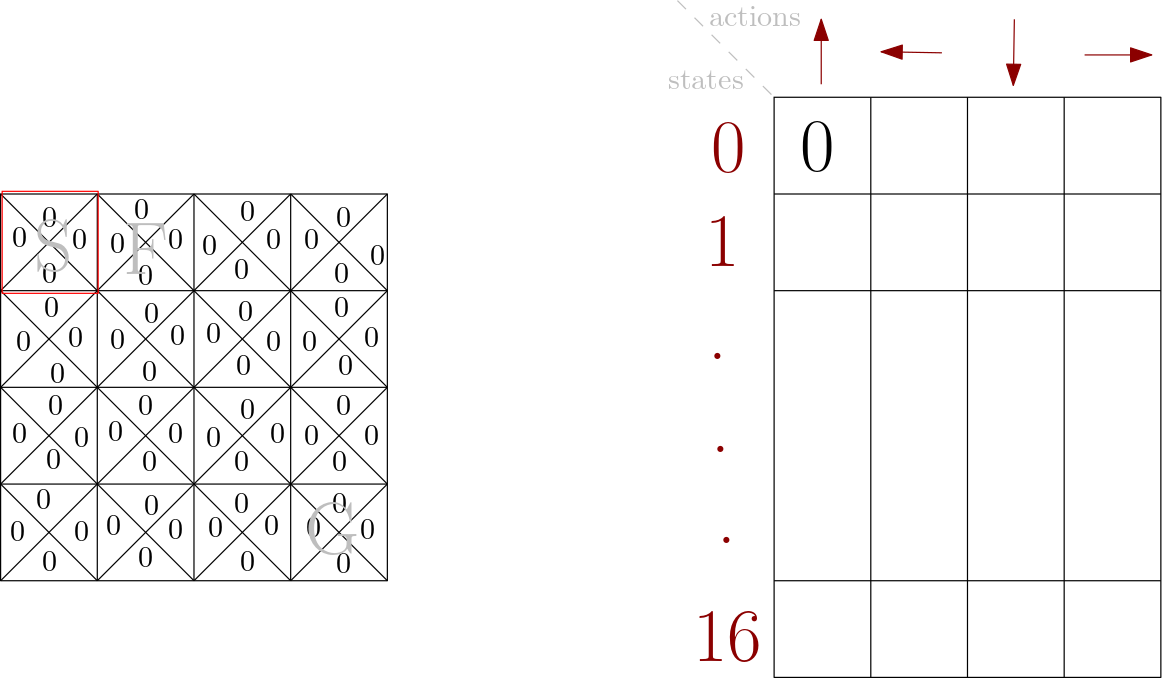
\includegraphics[width=9cm]{images/qtable.png}
\caption{Dve reprezentácie tej istej q-tabuľky pre FrozenLake - okienko predstavuje q(s,a).}
\end{figure}

\noindent Konkrétne, chceme aby agent volil akcie a na základe obdržaného rewardu update-oval hodnoty v tejto tabuľke:
\begin{figure}[H]
\centering
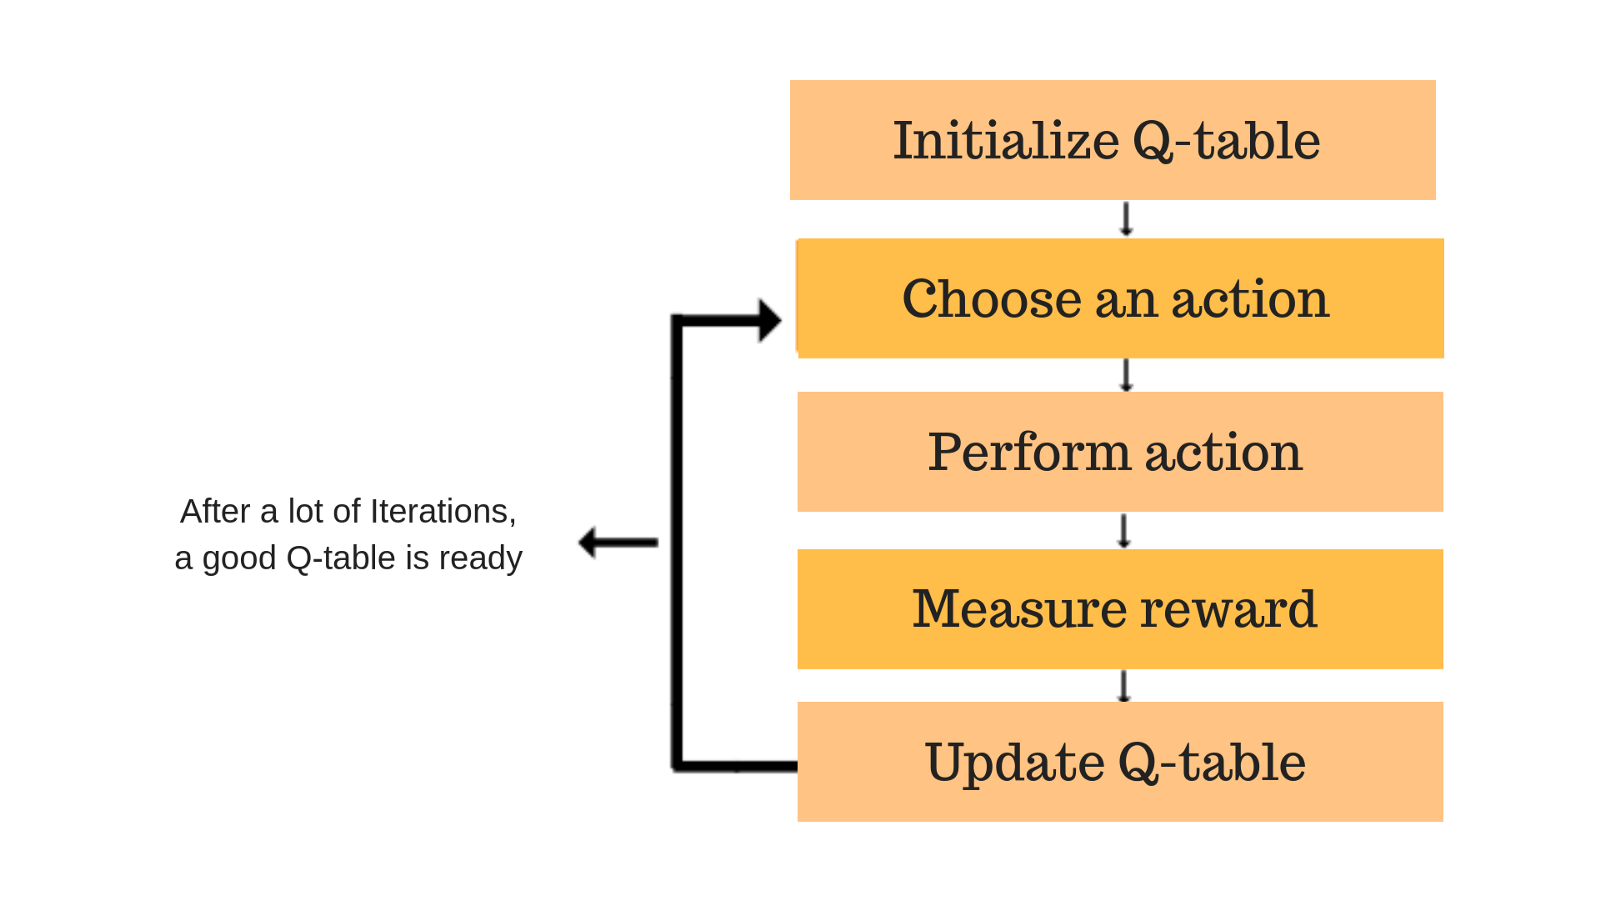
\includegraphics[width=11cm]{images/q-learning-scheme.png}
\caption{High-level schéma Q-learning algoritmu.}
\end{figure}

Akým spôsobom má ale agent voliť akcie? A ako sa má tento proces meniť s časom, keďže na začiatku agent o prostredí nevie nič ale postupne tieto vedomosti získava? Zaveďme teda koncept \textbf{exploration vs. exploitation}.

\textit{Explorácia} je proces, kedy skúmame prostredie a získavame o ňom nejaké informácie. V našom prípade to konkrétne znamená, že akciu budeme voliť náhodne. \textit{Exploitácia} je na druhú stranu proces, kedy využívame už zistenú informáciu o prostredí v snahe maximalizovať reward. Je teda zrejmé, že chceme začať exploráciou a postupne sa prepracovať k čistej exploitácii. Akým spôsobom to ale chceme urobiť?

Veľmi častá je tzv. \textbf{epilon greedy stratégia}. V nej sa zavádza \textbf{exploration rate} {\boldmath $\varepsilon$}, ktorý predstavuje pravdepodobnosť, s ktorým budeme v najbližšom kroku explorovať. Začíname s $\varepsilon = 1$ a postupne ho po krokoch/epizódach znižujeme. Často si ho ale zastavíme na nejakej hranici, napríklad $0.1$.
\vspace{0.4cm}
\begin{minted}[frame=single,framesep=10pt]{python}
# Exploration-exploitation trade-off
exploration_rate_treshold = random.uniform(0,1)
if exploration_rate_treshold > exploration_rate:
    action = np.argmax(q_table[state,:]) #"najväčší reward" (exploitácia)
else:
    action = env.action_space.sample() #náhodná akcia (explorácia)
\end{minted}
\vspace{0.3cm}

Už teda vieme ako voliť akcie. Akým spôsobom ale máme update-ovať hodnoty $q$-funkcie?
Podľa vedomostí získaných v prvej časti, vieme, že týmto krokom získaná hodnota danej q-funkcie, by mala byť
\begin{align*}
q(s,a) = r_{t+1} + \gamma \max\limits_{a'} q(s',a').
\end{align*}
My sme už ale čo-to o tejto hodnote zistili. Preto hodnotu q-funkcie update-ujeme nasledovne:
\begin{align*}
q^{new}(s,a) = (1 - \alpha) \cdot \underbrace{q(s,a)}_{old~value} + \alpha \cdot \overbrace{\big(r_{t+1} + \gamma \max\limits_{a'} q(s',a')\big)}^{learned~value}.
\end{align*} 
Čiže dávame nejakú váhu, konkrétne $1- \alpha$, predchádzajúcim vedomostiam.

\subsection{SARSA}
\subsection{Deep Q-learning network (DQN)}

\vspace{0.5cm}
\begin{minted}[frame=single,framesep=8pt]{python}
from keras.models import Sequential
from keras.layers import Dense
from keras.optimizers import Adam

# neural net to approximate Q-value function:
model = Sequential()
model.add( Dense(24, input_dim=state_size, activation='relu') )
model.add( Dense(24, activation='relu') )
model.add( Dense(action_size, activation='linear') )
model.compile(loss='mse', optimizer=Adam(lr=learning_rate))
\end{minted}




\section{Analýza}
TODO

\section{Záver}
TODO

%++++++++++++++++++++++++++++++++++++++++
% References section will be created automatically 
% with inclusion of "thebibliography" environment
% as it shown below. See text starting with line
% \begin{thebibliography}{99}
% Note: with this approach it is YOUR responsibility to put them in order
% of appearance.

% \begin{thebibliography}{99}

% \bibitem{melissinos}
% A.~C. Melissinos and J. Napolitano, \textit{Experiments in Modern Physics},
% (Academic Press, New York, 2003).

% \bibitem{Cyr}
% N.\ Cyr, M.\ T$\hat{e}$tu, and M.\ Breton,
% % "All-optical microwave frequency standard: a proposal,"
% IEEE Trans.\ Instrum.\ Meas.\ \textbf{42}, 640 (1993).

% \bibitem{Wiki} \emph{Expected value},  available at
% \texttt{http://en.wikipedia.org/wiki/Expected\_value}.

% \end{thebibliography}


\end{document}
